\chapter{BPM and jBPM}\label{bpm}

	\cite{bpm}
	Business process modeling (BPM), sometimes called business process management, refers to the design and execution of
	business processes.
	
	It does not have to be necessarily used in a context of \gls{IT} and software development. Primary field of BPM falls
	into management, though. Before \gls{ICT} was widely spread and automatic software processing was a dream, BPM was
	manual and paper driven.

	But yes, BPM is also closely aligned with the notion of \gls{SOA}, particularly the emerging W3C web services
	stack. Whereas the traditional use of a workflow was about the movement of work from person to person within an
	organization, contemporary BPM processes are built to interact as services with other systems, or even to orchestrate
	or choreograph other systems, including the business processes of other companies.

	\section{Business Process}

	A business process is a service, one intended to be called by other systems, and these calls drive its execution.
	Realizing this fact is one of the first big steps in understanding BPM.
	
	Being algorithmic, a process can potentially be run by some sort of process engine. As long as the process can be
	expressed in a form that is syntactically and semantically unambiguous that is, in a programming language or other
	interpretable form the engine can accept it as input, set it in motion, and drive its flow of control. To be precise,
	the engine creates and runs instances of a given process definition. The steps of the process are called activities or
	tasks.
	
	\section{Important process modelling terms}
	\begin{itemize}
		\item \textbf{Process definition}
		The basic algorithm or behavior of the process.
		\item \textbf{Process instance}
		An occurrence of a process for specific input. Each instance of the travel reservation process, for example, is tied
		to a specific customer's itinerary.
		\item \textbf{Activity or task}
		A step in a process, such as sending a flight request to the airline.
		\item \textbf{Automated activity or automated task}
		A step in a process that is performed directly by the execution engine.
		\item \textbf{Manual activity or manual task}
		A step in a process that is meant to be performed by a human process participant. 
	\end{itemize}
	
	The distinction between manual and automated activities is extremely important. At one time, before the reign of
	software, a business process was completely manual and paper-driven: paper was passed from person to person, and was
	often misplaced or delayed along the way. Now, much of the process runs on autopilot.

	Automated activities generally fall into two categories:
	\begin{itemize}
		\item \textbf{Interactions with external systems} e.g., sending a booking request to an airline
		\item \textbf{Arbitrary programmatic logic} e.g., calculating the priority of a manual task	   
	\end{itemize}
	
	\section{BPM application}
	
	BPM is suited only for applications with an essential sense of state or process that is, applications that are
	process-oriented. Typical characteristics of a process-oriented application are:
	
	\begin{itemize}
		\item \textbf{Long-running}
		From start to finish, the process spans hours, days, weeks, months, or more.
		\item \textbf{Persisted state}
		Because the process is long-lived, its state is persisted to a database so that it outlasts the server hosting it.
		\item \textbf{Bursty, sleeps most of the time}
		The process spends most of its time asleep, waiting for the next triggering event to occur, at which point it wakes up
		and performs a flurry of activities.
		\item \textbf{Orchestration of system or human communications}
		The process is responsible for managing and coordinating the communications of various system or human actors.
	\end{itemize}

	\section{BPM standards}
	
	BPM is not that difficult. The business analyst designs the process, the process is run by an engine, and the engine
	has EAI and human interaction capabilities. Questions appear when it comes to selection of a right solution, design and
	modelling tools, runtime engine, \ldots
	
	It is good to look for some well known and widely accepted approach. BPM does not lack standards. The adoption of
	\gls{BPEL} and \gls{BPMN} is a recipe for success. According to \cite[Ch.~1.3.1]{bpm}, the important BPM standards are:
	
	\begin{itemize}
		\item \gls{BPEL4WS}, sometimes shortened to \textbf{\gls{BPEL}}
		
		A BPEL process is a web service with an associated process definition defined in an XML-based language. The behavior
		of a BPEL process is to act on, and be acted on by, other processes; put differently, a BPEL process can invoke
		another web service or be invoked as a web service.
	  	\item \textbf{\gls{BPML}}
	  
		From the \gls{BPMI} organization, which is an XML-based process definition language similar to BPEL. BPMN, another
	  	specification from BPMI, is a sophisticated graphical notation language for processes. Significantly, the BPMN
	  	specification includes a mapping to BPML-rival BPEL, which facilitates the execution of BPMN-designed processes on
	  	BPEL engine.
	  	\item \textbf{Web services choreography}
	
	  	Choreography describes, from a global point of view, how web services are arranged in a control view spanning
	  	multiple participants. Choreography's global view is contrasted with the local view of process orchestration in
	  	languages such as BPEL; a BPEL process is the process of a single participant, and a choreography is the interaction
	  	model for a group of participants. \gls{WSCDL} is the W3C's recommended choreography standard.
	
	  	\item \gls{WfMC} has published a BPM reference model, as well as a set of interfaces for various parts of the BPM
	  	architecture. Though WfMC does not specify a standard graphical process notation, it does provide an exportable XML
	  	format called XML Process Definition Language (XPDL); processes built in an XPDL-compliant design tool can run on a
	  	WfMC enactment engine.
	  	
	  	\item \textbf{\gls{OMG}} did not aim build a new process language or interface but abstract BPM models conforming to
	  	its \gls{MDA}.
	  	\item \textbf{\gls{BPSS}} from OASIS group

	  	A choreography language, but is built for business-to-business collaborations. In a typical exchange between a buyer
	  	and seller, for example, the buyer sends a request to the seller, to which the seller responds immediately with
	  	consecutive acknowledgements of receipt and acceptance. When the seller has finished processing the request, it
	  	sends an indication of this to the buyer, and the buyer in turn sends an acknowledgement of the indication to the
	  	seller.
	\end{itemize}
	
	From the above are only two standards worth considering. BPEL and BPMN, which I am going to describe in analytical part
	of this work.

	\section{Execution engine - jBPM}
	
	\cite{jbpm}
	jBPM is a flexible \gls{BPM} Suite. It's light-weight, fully open-source (distributed under
	Apache license) and written in Java. It allows to model, execute and monitor business processes, throughout their life
	cycle.
	
	\begin{figure}[h]
	  	\centering
	    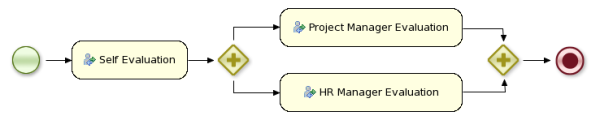
\includegraphics[width=12cm]{figures/jbpm_process.png}
	  	\caption{Example jBPM process as shown in \cite{jbpm}}
	\end{figure}
	
	A business process allows to model various business goals by describing the steps that need to be executed to achieve
	that goal and the order, using a flow chart. This greatly improves the visibility and agility of a business logic.
	jBPM focuses on executable business process, which are business processes that contain enough detail so they can
	actually be executed on a BPM engine. Executable business processes bridge the gap between business users and
	developers as they are higher-level and use domain-specific concepts that are understood by business users but can also
	be executed directly.

	The core of jBPM is a light-weight, extensible workflow engine written in pure Java that allows to execute business
	processes using the latest \gls{BPMN} 2.0 specification. It can run in any Java environment, embedded in an application
	or as a service.

	BPM makes the bridge between business analysts, developers and end users, by offering process management features and
	tools in a way that both business users and developers like it. Domain-specific nodes can be plugged into the palette,
	making the processes more easily understood by business users.

	jBPM supports adaptive and dynamic processes that require flexibility to model complex, real-life situations that
	cannot easily be described using a rigid process. jBPM is also not just an isolated process engine. Complex business
	logic can be modeled as a combination of business processes with business rules and complex event processing. jBPM can
	be combined with the Drools project to support one unified environment that integrates these paradigms where business
	logic can be modelled as a combination of processes, rules and events.

	Apart from the core engine itself, there are a few optional components that can be used. Eclipse-based or web-based
	business process designer and a management console for the execution engine.

	\subsection{jBPM Core Engine}
	
	The core jBPM engine is the heart of the jBPM project. It's a light-weight workflow engine that executes business
	processes.
	It can be embedded as a part of an application or deployed as a service. It's most important features are:
	
	\begin{itemize}
	  \item Solid, stable core engine for executing process instances
	  \item Native support for the latest BPMN 2.0 specification for modeling and executing business processes
	  \item Strong focus on performance and scalability
	  \item Light-weight (can be deployed on almost any device that supports a simple Java Runtime Environment, does not
	  require any web container at all)
	  \item (Optional) pluggable persistence with a default JPA implementation
	  \item Pluggable transaction support with a default JTA implementation
	  \item Implemented as a generic process engine, so it can be extended to support new node types or other process
	  languages
	  \item Listeners to be notified of various events
	  \item Ability to migrate running process instances to a new version of their process definition
	\end{itemize}

	The core engine can also be integrated with a few other (independent) core services:
	
	\begin{itemize}
	  \item The human task service can be used to manage human tasks when human actors need to participate in the process.
	  It is fully pluggable and the default implementation is based on the WS-HumanTask specification and manages the life
	  cycle of the tasks, task lists, task forms and some more advanced features like escalation, delegation, rule-based
	  assignments, etc.
	  \item The history log can store all information about the execution of all the processes on the engine. This is
	  necessary if access to historic information is needed as runtime persistence only stores the current state of all
	  active process instances. The history log can be used to store all current and historic state of active and completed
	  process instances.
	  
	  It can be used to query for any information related to the execution of process instances, for
	  monitoring, analysis, etc.
	\end{itemize}
